\section{Analysis \& Comparisons}
\subsection{Simulation Overview \& Governing Equations}

The governing equations for the DNS of compressible turbulent channel flows are:

\begin{align}
  %NS DNS eqns
  \frac{\partial \rho}{\partial t}+\frac{\partial (\rho u_i)}{\partial x_i}           & = 0                                                                                                           \\[.5ex] % continuity
  \frac{\partial (\rho u_i)}{\partial t}+\frac{\partial (\rho u_i u_j)}{\partial x_j} & =-\frac{\partial p}{\partial x_i}+\frac{\partial \sigma_{i j}}{\partial x_j}+f \delta_{i 1} x \label{eqn:mom} \\[.5ex] % NS, f term is forcing function to enforce mom conservation
  \frac{\partial (\rho E)}{\partial t}+\frac{\partial (\rho u_j H)}{\partial x_j}     & =-\frac{\partial q_j}{\partial x_j}+\frac{\partial (\sigma_{i j} u_i)}{\partial x_j}+f u_1 \label{eqn:eng}    % energy, f here is for enforcing energy conservation
\end{align}

Where the $f$ terms in \Cref{eqn:mom} and \Cref{eqn:eng} serve to enforce a constant mass flow rate in time and $\delta_{ij}$ is the Kronecker delta \cite{modestiReynoldsMachNumber2016}. The stress tensor and thermodynamic variables are defined as:

\begin{align}
  \sigma_{i j} & =\mu\left(\frac{\partial u_i}{\partial x_j}+\frac{\partial u_j}{\partial x_i}-\frac{2}{3} \frac{\partial u_k}{\partial x_k} \delta_{i j}\right) \\[.5ex] %stress tensor
  q_j          & =-k \frac{\partial T}{\partial x_j}                                                                                                             \\[.5ex] %heat
  E            & =c_v T+u_i u_i / 2                                                                                                                              \\[.5ex] %energy E
  H            & =E+p / \rho                                                                                                                                     %enthalpy
\end{align}

For an idea on how expensive DNS is, Pope states that the explicit timestep is roughly on the order of 10\% of the Kolmogorov time scale and the minimum grid spacing is of the order of the Kolmogorov length scale. If we relate this to results we have seen in class, we get a simplistic but informative estimation of the DNS cost.

\begin{align*} %dns grid
  \Delta x & \sim  2.5 \ \eta,  \ \eta \sim Re^{-3/4}         \\
  \Delta t & \sim  .1 \ \tau_\eta, \ \tau_\eta \sim Re^{-1/2}
\end{align*}

\subsection{Transformation Results}
In this section the compressible and incompressible DNS results for the four different transformations studied by Modesti \& Pirozzoli are displayed.
\subsubsection{Velocity Comparison}
The equivalent friction Reynolds number is defined as $Re_{\tau_i} = \frac{\delta(y_i)}{\delta_\nu}$, where $\delta(y_i)$ is the characteristic length scale after applying the y coordinate transformation.  Notice that all cases are for Mach 1.5, except for the bottom right figure in a set, which is at Mach 3. Performance of the transformation is registered as its ability to collapse the compressible turbulence profiles to the incompressible profiles. First, observing the classic Van Driest transformation in \Cref{fig:v-vd}, we see poor performance at all Reynolds numbers (notice $Re_\tau$ and $Re_{\tau_D}$ are identical). The compressible velocity profile varies the most at the low Reynolds number case and performance of the transformation is exacerbated by an increase in the Mach number.

\begin{figure}[h]
  \centering
  \setlength{\abovecaptionskip}{20pt}

  \begin{tabular}{
    >{\centering\arraybackslash}m{.30\textwidth}  @{\quad}
    >{\centering\arraybackslash}m{.50\textwidth}
    }
    % Row 1: the two images, each centered in a fixed‐height cell
    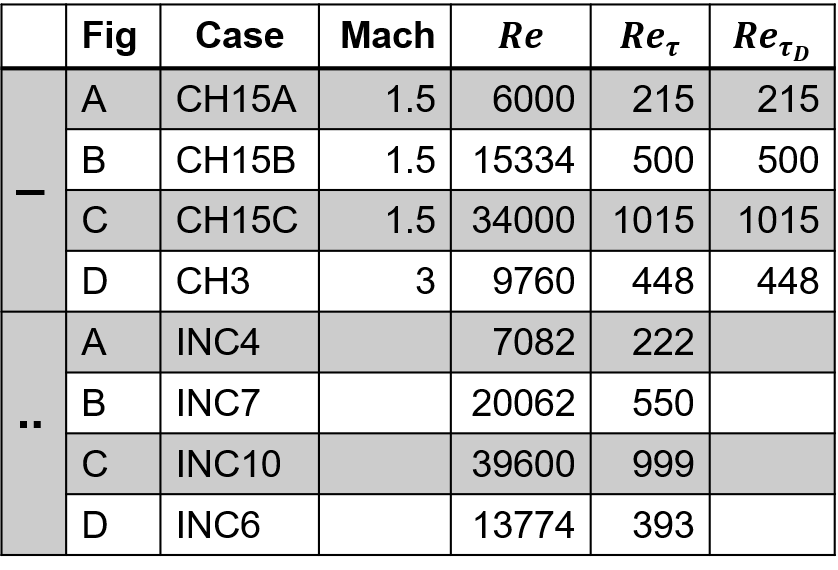
\includegraphics[width=\linewidth]{images/van-driest-mean-table.png}
     &
    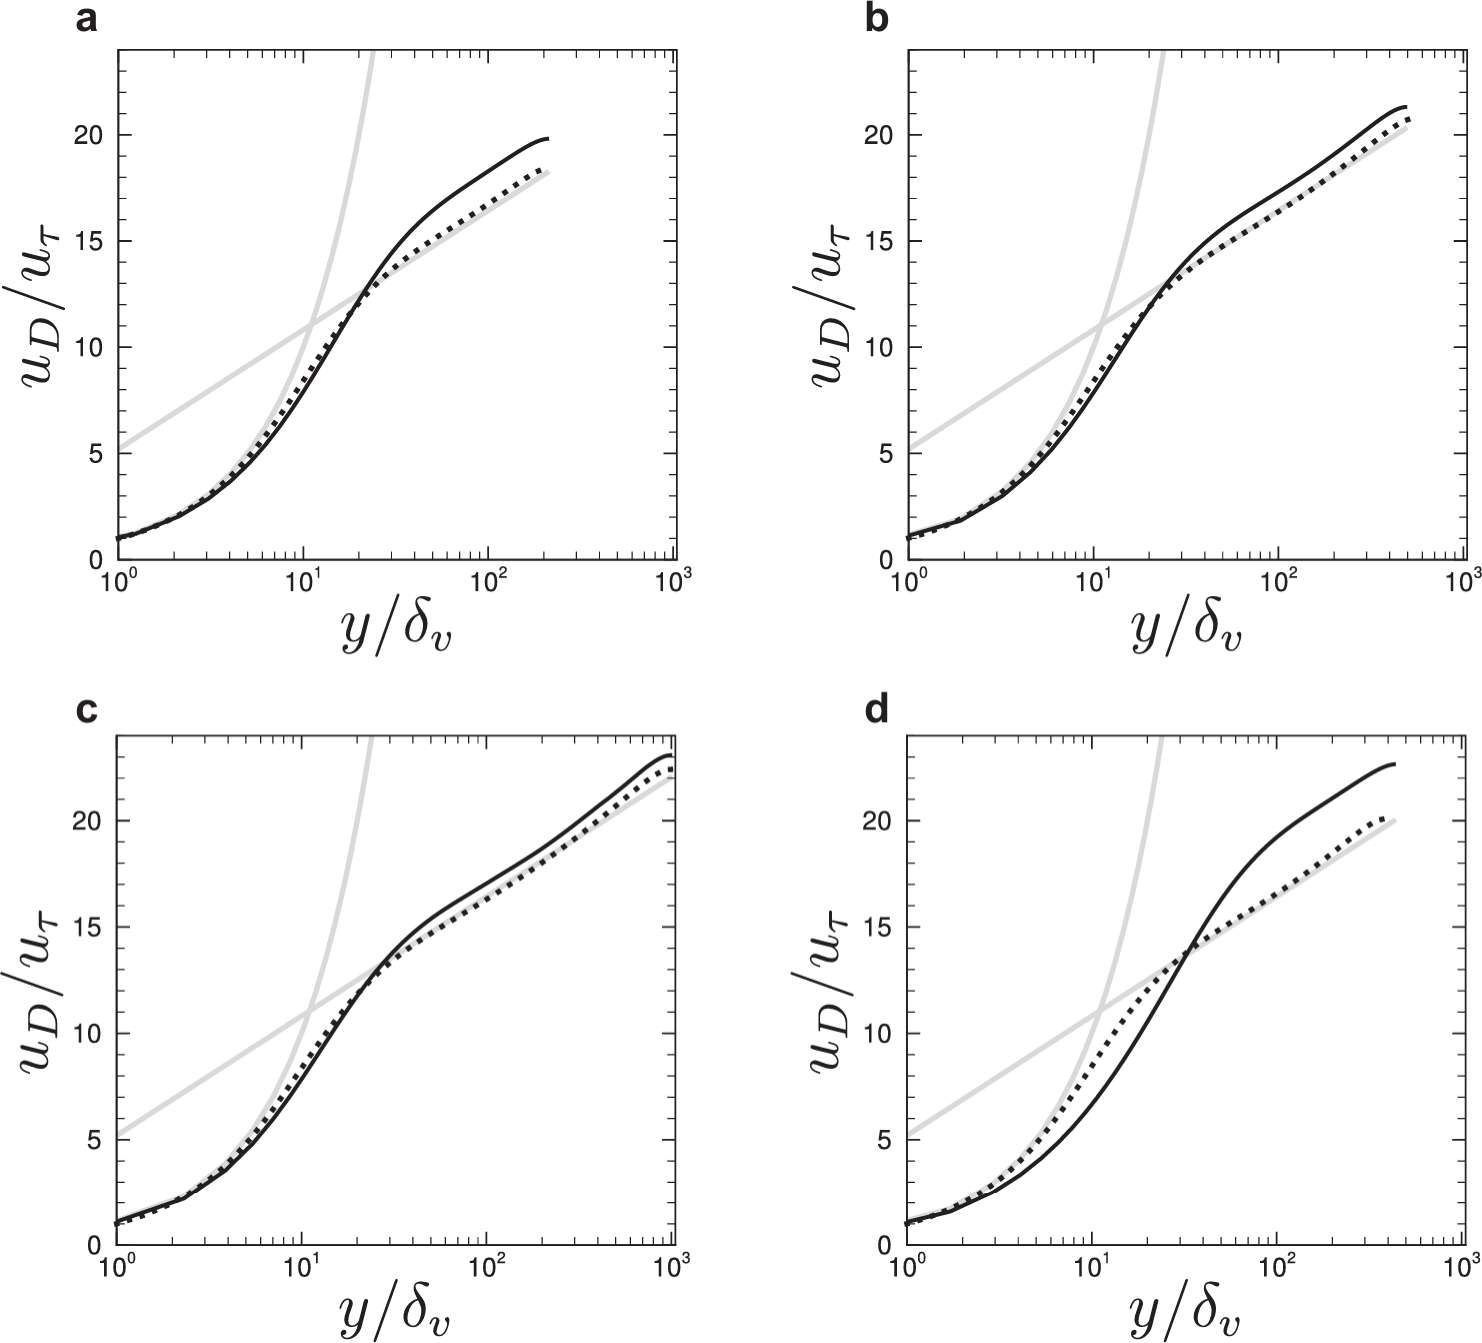
\includegraphics[width=\linewidth]{images/van-driest-incomp-compare1.png}
    \\[1ex]
    % Row 2: the two sub‐captions, same baseline
    (a) Conditions
     &
    (b) Velocity profiles
  \end{tabular}

  \caption{\label{fig:v-vd}
    Velocity comparison of compressible (solid black) to incompressible (black dots) DNS
    using Van Driest transformation taken from Modesti \& Pirozzoli \cite{modestiReynoldsMachNumber2016}}
\end{figure}



\subsubsection{Reynolds Stress Comparison}
Next, the Reynold's stress components are compared for each compressibility transformation. The scaling arguments utilized in the Van Driest, Huang, and Trettel \& Larsson transformations all yield a simple transformation that can be applied to each Reynolds stress component, $\tau_{ij} \Rightarrow \frac{\langle \rho \rangle}{\langle \rho_w \rangle}\tau_{ij}$. Brun's transformation yields a slightly different result for the diagonal components of the Reynolds stress tensor, $\tau_{{ii}_B} = \frac{\langle \rho \rangle}{\langle \rho_w \rangle}(\frac{y}{y_B}\frac{\langle \mu_w \rangle}{\langle \mu \rangle})^2 \tau_{ii}$. The format of the comparisons is the same as the mean velocity transformations. First, Van Driest's transformation is shown in \Cref{fig:r-vd}.

\begin{figure}[ht]
  \centering
  \setlength{\abovecaptionskip}{20pt}

  \begin{tabular}{
    >{\centering\arraybackslash}m{.30\textwidth}  @{\quad}
    >{\centering\arraybackslash}m{.50\textwidth}
    }
    % Row 1: the two images, each centered in a fixed‐height cell
    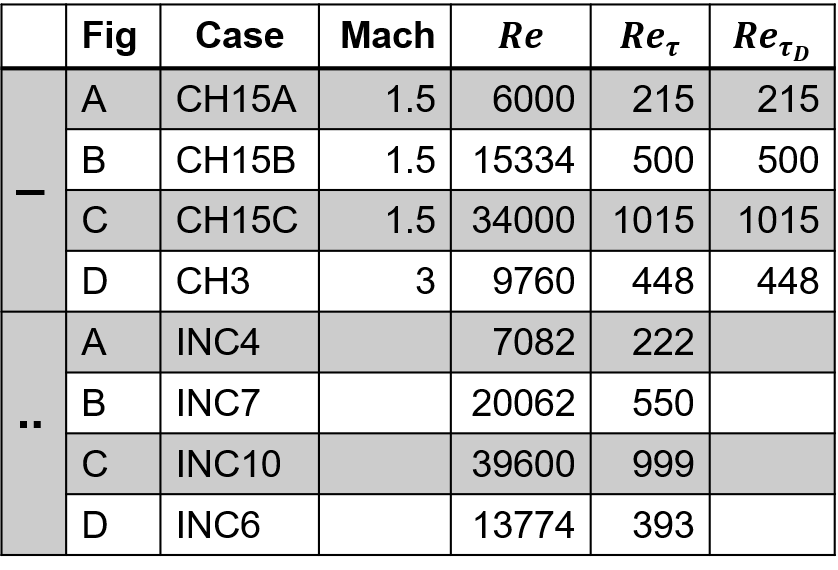
\includegraphics[width=\linewidth]{images/van-driest-reynolds-table.png}
     &
    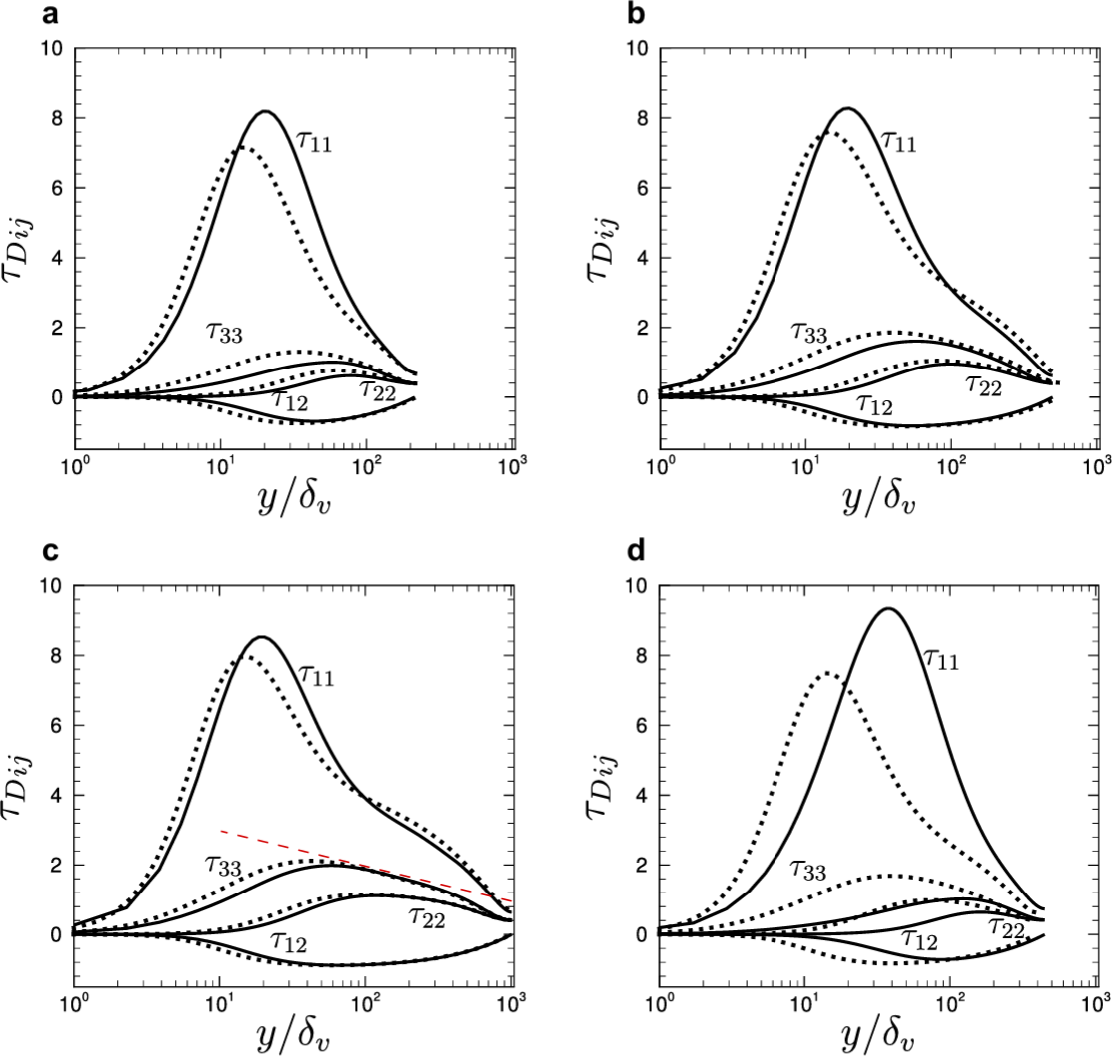
\includegraphics[width=\linewidth]{images/van-driest-incomp-compare2.png}
    \\[1ex]
    % Row 2: the two sub‐captions, same baseline
    (a) Conditions
     &
    (b) Reynolds stress profiles
  \end{tabular}

  \caption{\label{fig:r-vd}
    Reynolds stress comparison of compressible (solid black) to incompressible (black dots) DNS using Van Driest transformation taken from Modesti \& Pirozzoli \cite{modestiReynoldsMachNumber2016}}
\end{figure}